\documentclass[12pt]{article}


\usepackage[utf8]{inputenc}
\usepackage[a4paper,top=3cm,bottom=2cm,left=3cm,right=3cm,marginparwidth=1.75cm]{geometry}
\usepackage[nodayofweek]{datetime}
\usepackage{tabularx}
\usepackage[small]{titlesec}
\usepackage{graphicx}
\usepackage{tabularx}

\newcolumntype{L}[1]{>{\raggedright\arraybackslash}p{#1}}
\newcolumntype{C}[1]{>{\centering\arraybackslash}p{#1}}
\newcolumntype{R}[1]{>{\raggedleft\arraybackslash}p{#1}}

\begin{document}

\begin{titlepage}
    \begin{center}
        \huge{\bfseries  Tribhuvan University}\\
        \Large{Institute of Engineering}\\
        \huge{ \bfseries  Pulchowk Campus}\\[3.2cm]


        \textsc{\Large Internet and Intranet}\\[-0.5cm]
        \line(1,0){400}\\
        \huge{\bfseries Lab 1}\\
        \large{VSFTP Server Configuration}
        \line(1,0){400}\\


        \textsc{\Large Submitted by:}\\
        \Large Bishal Katuwal\\ \large 075BCT028\\    [0.85cm]

        \textsc{\Large Submitted to:}\\\
        \large Department of Electronics and Computer Engineering\\Pulchowk Campus\\    [0.85cm]
        
        \textsc{\Large Submitted on:}\\
        \today
        
    \end{center}
\end{titlepage}
\pagebreak
% ===============================================================
\paragraph{\Large Title\\}
VSFTP Server Configuration

\paragraph{Background Theory\\}
File transfer protocol (FTP) is a standard network protocol 
used for the transfer of files from one host to another over 
a TCP-based network, such as the Internet. FTP is a commonly 
used protocol for transferring files between computers, and 
it is also used to transfer files from a server to a client 
or from a client to a server. One of the most popular and 
secure FTP server software is VSFTP (Very Secure File Transfer 
Protocol).

VSFTP(Very Secure FTP) is a free and open-source FTP server software 
that is widely used on Linux and Unix-based operating systems, as well 
as Windows. 
It offers a variety of features including support for virtual users, 
SSL/TLS encryption, and file permissions. VSFTP is considered to be 
one of the most secure FTP servers available, and it is often used 
for securely transferring files over a network. In this report, 
we will discuss the basic steps to install and configure a VSFTP 
server on Linux and Windows operating systems.

\paragraph{Activity}
\section{VSFTPD Installation}
\begin{enumerate}
    \item Updated system packages.
    \begin{verbatim}
        sudo apt update
    \end{verbatim}
    \item Installed VSFTPD package.
    \begin{verbatim}
        sudo apt install vsftpd ftp ufw -y 
    \end{verbatim}
    \item Enabled the VSFTPD server.
    \begin{verbatim}
        sudo systemctl enable vsftpd
    \end{verbatim}
    \item Launched VSFTPD.
    \begin{verbatim}
        sudo systemctl start vsftpd
    \end{verbatim}
    \item Checked the status of VSFTPD.
    \begin{verbatim}
        sudo systemctl status vsftpd
    \end{verbatim}
\end{enumerate}
\begin{figure}
    \centering
    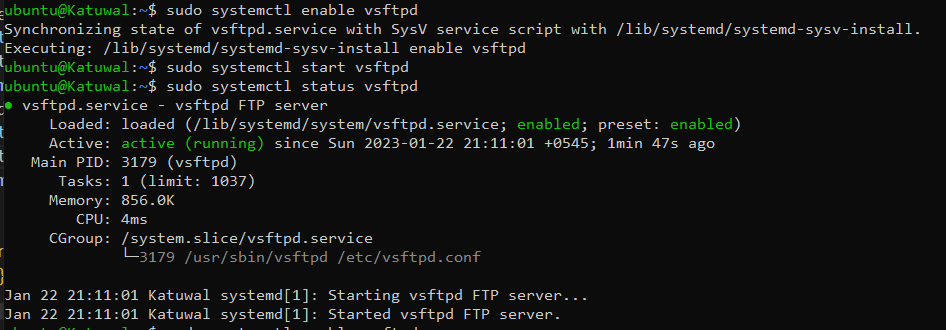
\includegraphics[scale = 0.70]{Images/Setup.PNG}
    \caption{VSFTPD installation}
\end{figure}
\section{Configuration file for VSFTPD}
\begin{enumerate}
    \item VSFTPD file was configurde as follows.
    \begin{verbatim}
log_ftp_protocol=YES
anonymous_enable=YES # allow anonymous user to login
seccomp_sandbox=NO # this line disables security sandbox
use_sendfile=YES # enable send/receive file functionality
local_enable=YES # allow local users to login
write_enable=YES # allow FTP write command
anon_upload_enable=YES # allow anonymous users to upload
dirmessage_enable=YES
xferlog_enable=YES
connect_from_port_20=YES
listen=YES
pam_service_name=vsftpd

    \end{verbatim}
    \item VSFTPD was restarted.
    \begin{verbatim}
    sudo systemctl restart vsftpd
    \end{verbatim}
\end{enumerate}
\begin{figure}[h!]
    \centering
    
\includegraphics{Images/restart.PNG}
    \caption{VSFTPD restart}
\end{figure}
\section{FTP Connection}
\begin{enumerate}
    \item Connect using ftp IP
    \item Use recv to receive and send to send.
    \begin{verbatim}
        ftp localhost
        ls
        recv test.txt
    \end{verbatim}
\end{enumerate}
\paragraph{Conclusion\\}
In this report, we have discussed the basic steps to install and 
configure a VSFTP server on Linux operating systems. 
The process of configuring a VSFTP server involves installing the 
software, configuring the settings, creating virtual users, and 
testing the server to ensure it is working properly.

\end{document}